\chapter{Related Work}
\label{chap:related-work}

Genomics is a field that has been growing rapidly in the past few years. The advent of high-throughput
sequencing technologies has made it possible to sequence the entire genome of an organism in a matter
of days. This has led to an explosion of data, with the number of sequenced genomes increasing exponentially.
This has created a need for new tools and algorithms to analyze this data. In this chapter, we review
some of the existing tools and algorithms for analyzing genomic data.

\section{Genomic data analysis}
\label{sec:genomic-data-analysis}

\subsection*{Random forests}
\label{subsec:random-forests}

Another method that has been used for genomic data analysis is random forests (RF) \cite{Chen-Ishwaran-2012}.
This method is based on the idea of ensemble learning, where multiple decision trees are trained on different
subsets of the data and then combined to make a final prediction.

\subsection*{AI applications in genomic analysis}
\label{sec:ai-applications-in-genomic-analysis}

Many researchers have used AI techniques to analyze genomic data. For example, \cite{Caudai-et-al-2021} reviews
different AI techniques that have been used for genomic data analysis, including CNNs, autoencoders, etc.

More recently, the authors of \cite{Zhou-et-al-2024} designed a tool based on multiple LLM backends for multi-omics
analysis with minimal human intervention.

\section{Introduction to CNNs}
\label{sec:intro_cnn}

The fundamental idea behind \textbf{Convolutional Neural Networks (CNNs)} was introduced by Kunihiko Fukushima\textsuperscript{\cite{Fukushima-1987}}
in 1980 and later popularized by Yann LeCun in the 1990s with the LeNet architecture\textsuperscript{\cite{Lecun-et-al-1998}}. CNNs are a class of
deep learning models specifically designed for processing structured grid data, such as images. They are particularly effective for
tasks like image classification, object detection, and segmentation.

CNNs work by applying convolutional filters to the input data, which allows them to learn spatial hierarchies of features.
It shares some similarities with the more conventional neural networks, but there is at least two different types
of layers that are specific to CNNs:

\begin{itemize}
	\item \textbf{Convolutional layers}: These layers apply convolutional filters to the input data, extracting local features
	      that are invariant to translation. The filters slide over the input data, computing dot products and producing feature maps.
	\item \textbf{Pooling layers}: These layers downsample the feature maps, reducing their spatial dimensions while retaining important
	      information. Common pooling operations include max pooling and average pooling.
\end{itemize}

The architecture of a CNN typically consists of multiple convolutional and pooling layers followed by fully connected layers.
The convolutional layers learn to extract features from the input data, while the fully connected layers perform the final classification
or regression task. The training process involves optimizing the weights of the filters and fully connected layers using backpropagation
and a loss function, such as cross-entropy for classification tasks.

\subsubsubsection{K-fold cross validation}
\label{subsubsec:k_fold_cross_validation}

K-fold cross validation is a specific type of cross validation where the dataset is divided into $k$ equally sized folds. The model is trained
on $k-1$ folds and tested on the remaining fold, and this process is repeated for each fold. The final performance is averaged over all folds
to obtain a more reliable estimate of the model's performance. The graphical representation of K-fold cross validation is shown in Figure~\ref{fig:k_fold}.

\begin{figure}[htbp]
	\centering
	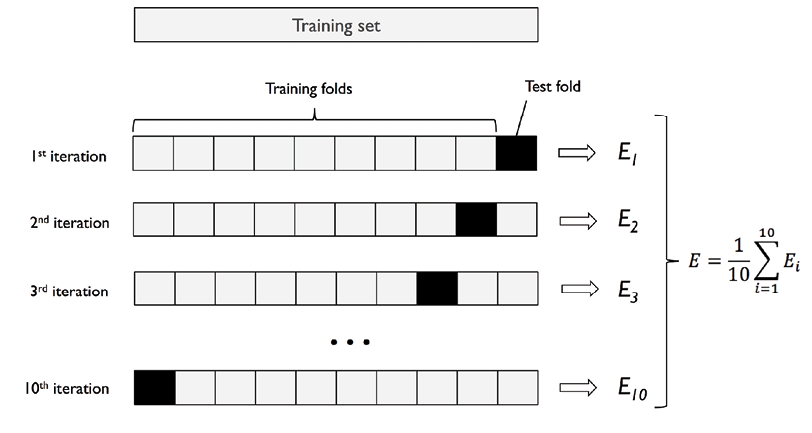
\includegraphics[width=0.8\textwidth]{../imgs/kfold.png}
	\caption{How K-fold cross validation works.\textsuperscript{\cite{Raschka-Mirjalili-2017}}}
	\label{fig:k_fold}
\end{figure}

\subsubsubsection{Stratified K-fold cross validation}
\label{subsubsec:stratified_k_fold_cross_validation}

Stratified K-fold cross validation is a variation of K-fold cross validation that ensures that each fold has the same proportion of samples
from each class. This is particularly useful for imbalanced datasets, as it ensures that each fold has a representative sample of each class.
Even if this method is recommended for imbalanced datasets, we did not have enough time to implement it, so we used the standard K-fold cross
validation.

\subsubsubsection{SMOTE}
\label{subsubsec:smote}

Data augmentation is a technique used to artificially increase the size of a dataset by applying various transformations to the existing data.
This can help improve the model's performance by providing more diverse training samples and reducing overfitting. In our project, we used SMOTE
(Synthetic Minority Over-sampling Technique) to generate synthetic samples for the minority classes in our dataset.

SMOTE works by creating new samples by interpolating between existing samples in the feature space. It generates synthetic samples by selecting
a minority class sample, finding its nearest neighbors, and creating new samples by interpolating between the selected sample and its neighbors.
This helps to balance the dataset by increasing the number of samples in the minority classes, which can improve the model's performance on those
classes.

New samples are generated by taking a random sample from the minority class and finding its nearest neighbors in the feature space. The new sample
is then created by interpolating between the selected sample and its neighbors, as shown in Figure~\ref{fig:smote}. It uses the following formula:

\begin{equation}
	x_{new} = x_{i} + \lambda (x_{j} - x_{i})
\end{equation}

Where $x_{new}$ is the new sample, $x_{i}$ is the selected sample, $x_{j}$ is one of its nearest neighbors, and $\lambda$ is a random number
between 0 and 1. This process is repeated until the desired number of samples is generated for the minority class.

\begin{figure}[htbp!]
	\centering
	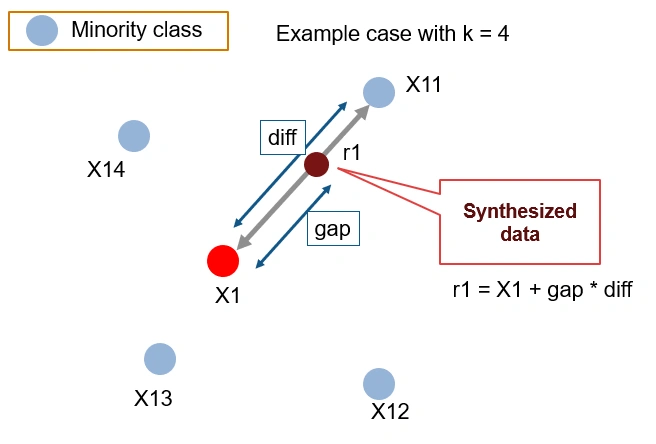
\includegraphics[width=0.6\textwidth]{../imgs/smote.png}
	\caption{Illustration of the SMOTE algorithm.\textsuperscript{\cite{analyticsvidhya-2020}}}
	\label{fig:smote}
\end{figure}